\begin{figure}[H]
    \centering
    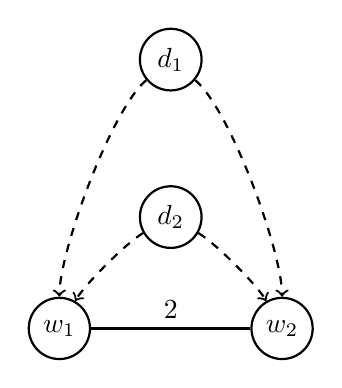
\begin{tikzpicture}[node distance=2cm, thick, main/.style = {draw, circle}]
        \node[main] (1) [] {$d_1$};
        \node[main] (2) [below of=1] {$d_2$};
        \node[main] (3) [below left of=2] {$w_1$};
        \node[main] (4) [below right of=2] {$w_2$};
        \draw[->] (1) to [out=220, in=90, looseness=0.5] (3) [dashed] node {};
        \draw[->] (1) to [out=320, in=90, looseness=0.5] (4) [dashed] node {};
        \draw[->] (2) to [out=210, in=60, looseness=0.5] (3) [dashed] node {};
        \draw[->] (2) to [out=330, in=120, looseness=0.5] (4) [dashed] node {};
        \draw[] (3) -- node[midway, above] {2} (4);
    \end{tikzpicture}
    \caption{Co-Occurrence} \label{fig:co_occurrence}
\end{figure}
